\chapter{End-to-End Mathematical Audit Trail}
\label{appendix:math_trail}

This appendix provides a complete, step-by-step visual breakdown of the Verification Audit for the Python metric, as calculated by the MERIT execution engine. This explicitly details the underlying mathematical logic including temporal decay, heuristic normalisation, Bayesian Evidence Fusion, and Shapley Value attribution.

\begin{figure}[htpb]
    \centering
    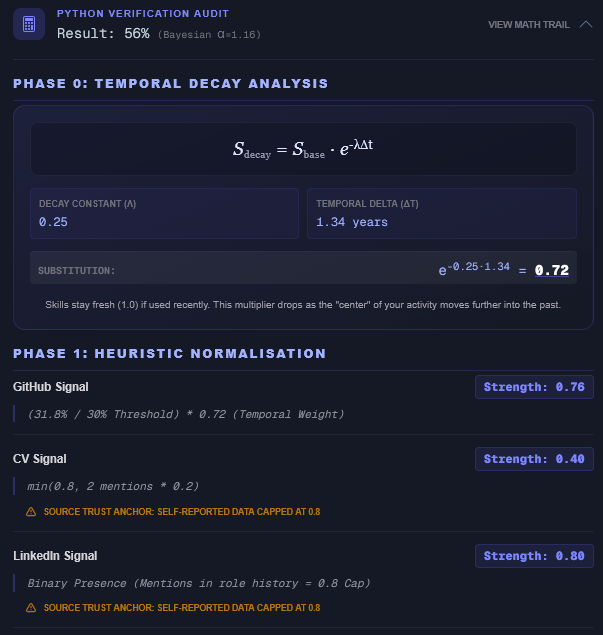
\includegraphics[width=0.85\textwidth]{implementation/screenshots/math_trail_phase_0_1.png}
    \caption{Phase 0 and Phase 1 of the Verification Audit for the a Python metric (extensible metric derived from a JD). 
    The math trail explicitly shows the application of the temporal decay penalty 
    and the heuristic normalisation of signals from the candidate's GitHub, CV, and LinkedIn.}
    \label{fig:audit_trail_phase_1}
\end{figure}

\begin{figure}[htpb]
    \centering
    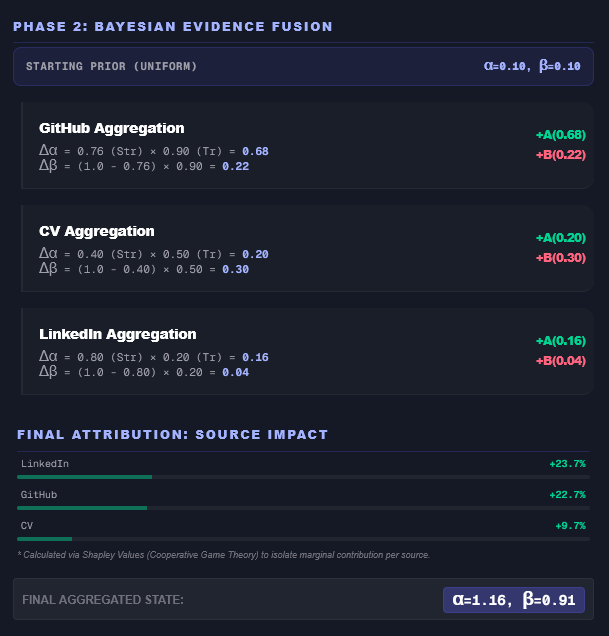
\includegraphics[width=0.85\textwidth]{implementation/screenshots/math_trail_phase_2.png}
    \caption{Phase 2 of the Verification Audit, visualising the Bayesian Evidence Fusion 
    process. It also displays the final attribution of source impact for this specific metric, 
    calculated via Shapley Values.}
    \label{fig:audit_trail_phase_2}
\end{figure}

\begin{figure}[htpb]
    \centering
    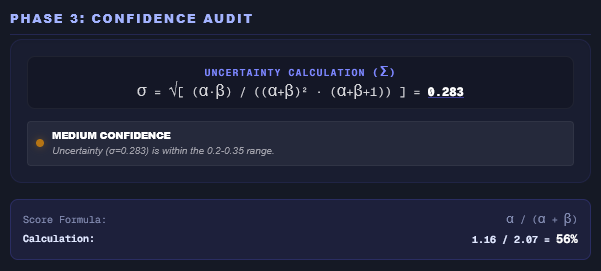
\includegraphics[width=0.85\textwidth]{implementation/screenshots/math_trail_phase_3.png}
    \caption{Phase 3 of the Verification Audit, where the mathematical uncertainty ($\sigma$) 
    of the Beta distribution is calculated to derive the final confidence level of the metric's score.}
    \label{fig:audit_trail_phase_3}
\end{figure}
